\clearpage
\section{Upsampling-factor and POD-rank sensitivity}
\label{app:qr_sensitivity}

This appendix examines the fixed interpolation factor $q$ and POD rank $r$ used by the assisted preprocessors. For PDEs, the $q=1$ column is a POD-only denoising control: the noisy sparse snapshots are projected to rank $r$ and reconstructed at the observed times, but no temporal points are inserted. Values with $q>1$ combine the same POD projection with DMD/EDMD temporal upsampling. The study is not used for oracle selection in the main tables; it is a representative robustness check at the same synthetic-equation level. Unless otherwise stated, the sensitivity run uses relative noise 0.03, ODE sparse factor 16, PDE sparse factor 8, and 5 random seeds.

\begin{figure}[H]
\centering
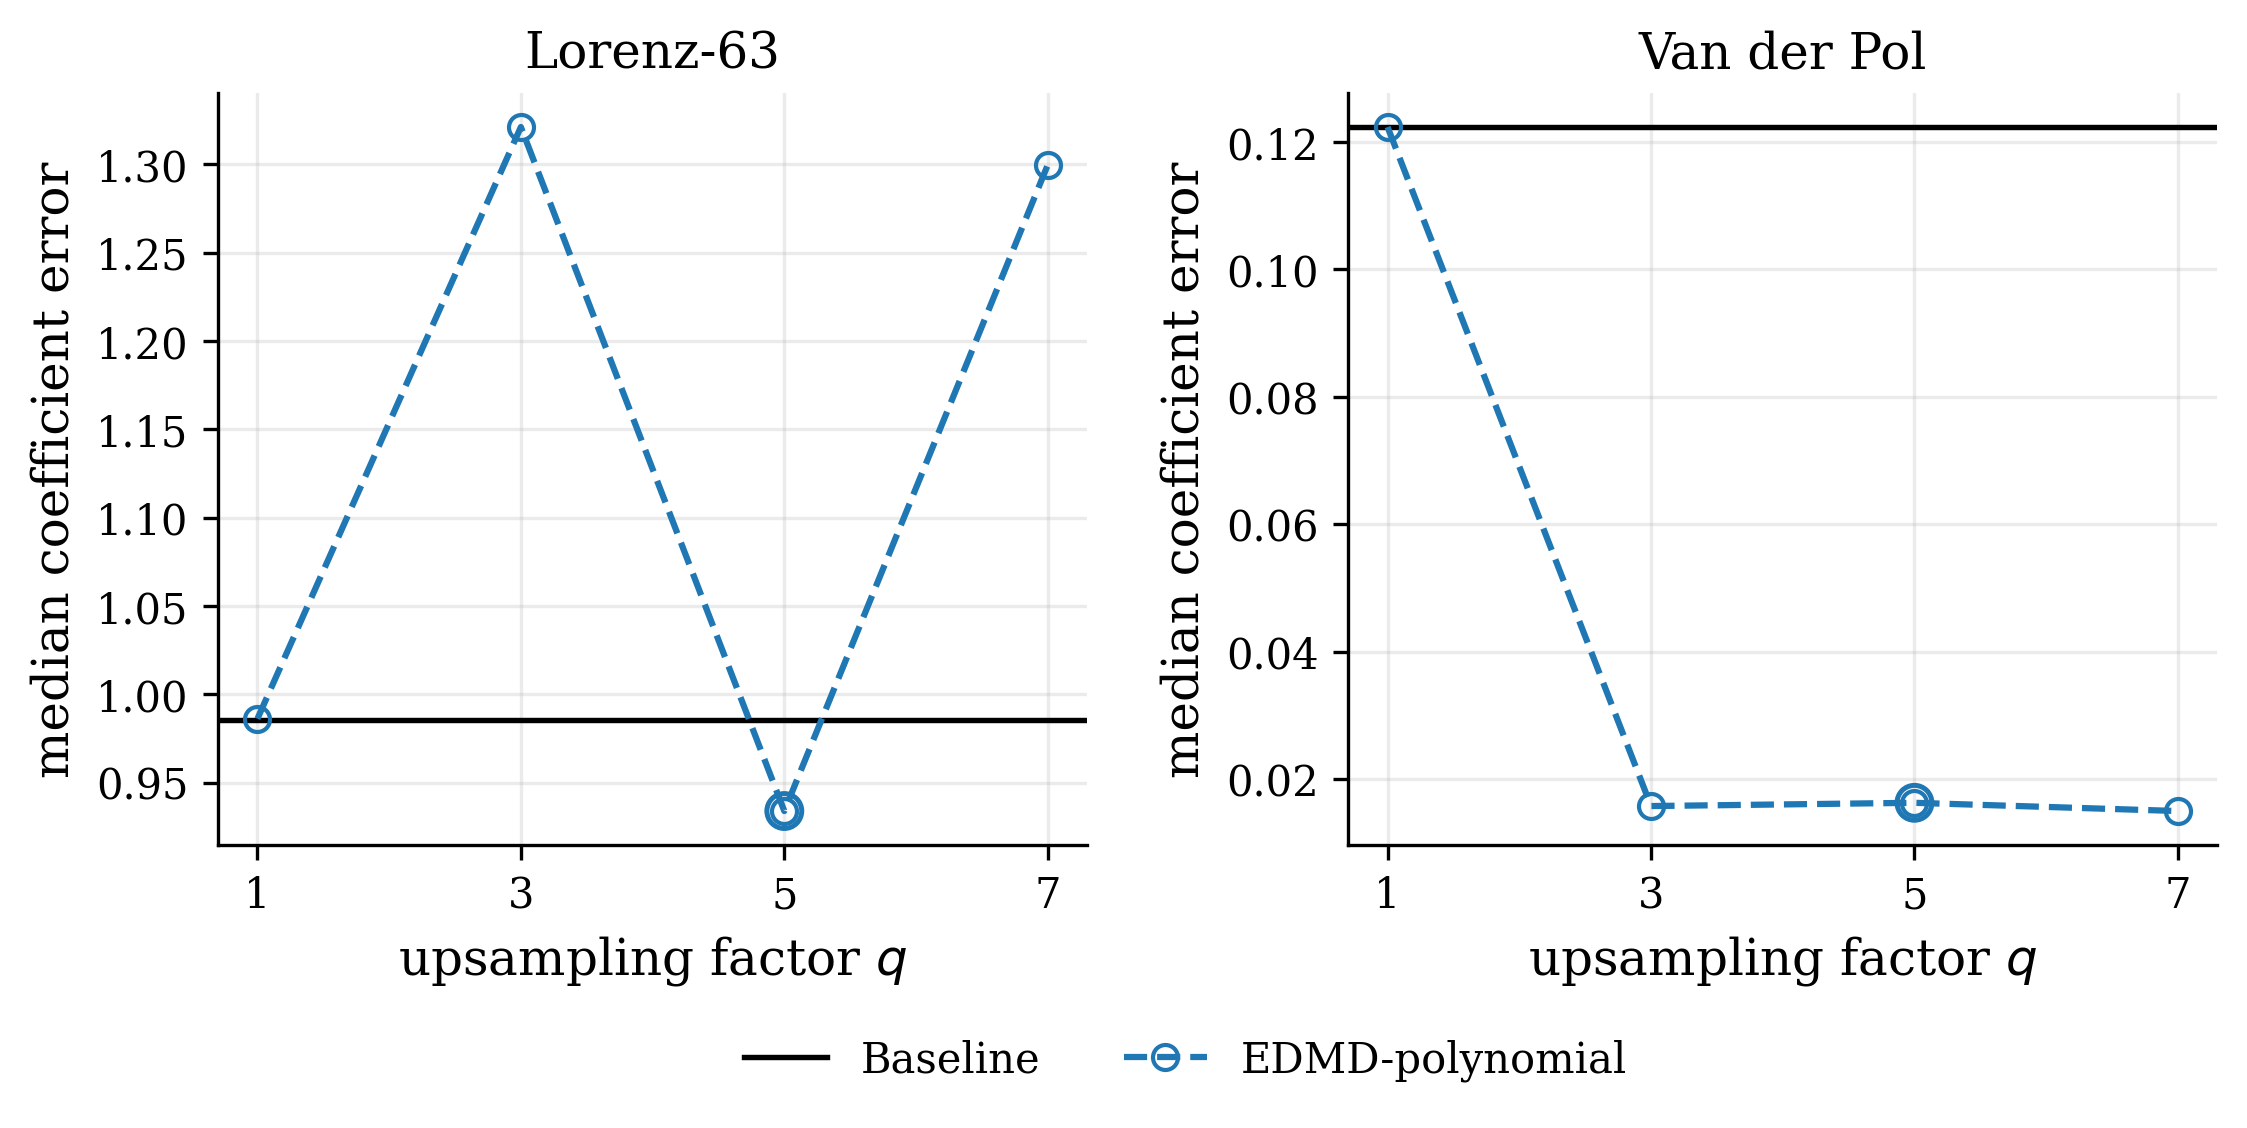
\includegraphics[width=0.95\textwidth]{figures/appendix_q_sensitivity_ode.png}
\caption{ODE sensitivity to the upsampling factor $q$ for EDMD-polynomial preprocessing. Horizontal black lines show the no-upsampling baseline; dashed blue curves show EDMD-polynomial. Markers at $q=5$ indicate the value used in the main benchmark.}
\label{fig:appendix_q_sensitivity_ode}
\end{figure}

\begin{table}[H]
\centering
\TBL{\caption{ODE $q$ sensitivity for Lorenz--63 and Van der Pol under EDMD-polynomial preprocessing. The sensitivity run uses relative noise 0.03, sparse factor 16, and five random seeds. F1 and practical score are means; coefficient error is the median over valid evaluation records. Boldface marks the best value at reported precision within each system.\label{tab:appendix_ode_q_sensitivity}}}
{\begin{tabular}{@{}llcccc@{}}\toprule
\TCH{System} & \TCH{Method} & \TCH{$q$} & \TCH{F1} & \TCH{Coeff. err.} & \TCH{Score} \\ \midrule
Lorenz--63 & Baseline & -- & 0.554 & 0.986 & 0.268 \\
 & EDMD-polynomial & 1 & 0.562 & 0.986 & 0.272 \\
 & EDMD-polynomial & 3 & 0.591 & 1.321 & 0.261 \\
 & EDMD-polynomial & 5 & 0.563 & \textbf{0.934} & \textbf{0.288} \\
 & EDMD-polynomial & 7 & \textbf{0.609} & 1.300 & 0.273 \\
\midrule
Van der Pol & Baseline & -- & \textbf{1.000} & 0.122 & 0.893 \\
 & EDMD-polynomial & 1 & \textbf{1.000} & 0.122 & 0.893 \\
 & EDMD-polynomial & 3 & \textbf{1.000} & 0.016 & 0.982 \\
 & EDMD-polynomial & 5 & \textbf{1.000} & 0.016 & \textbf{0.984} \\
 & EDMD-polynomial & 7 & \textbf{1.000} & \textbf{0.015} & \textbf{0.984} \\
\botrule
\end{tabular}}
\end{table}

Figure~\ref{fig:appendix_q_sensitivity_ode} and Table~\ref{tab:appendix_ode_q_sensitivity} show that the usefulness of increasing $q$ is system-dependent. For Van der Pol, EDMD-polynomial is already substantially better than the baseline for $q\geq3$, and the default $q=5$ is near the best observed value. For Lorenz--63, the sensitivity is less monotone, which is consistent with the chaotic trajectory and the difficulty of estimating accurate derivatives from sparse noisy measurements. The default $q=5$ gives the lowest median coefficient error among the EDMD-polynomial values tested for Lorenz--63, although the practical score varies only modestly across the grid.

\begin{figure}[H]
\centering
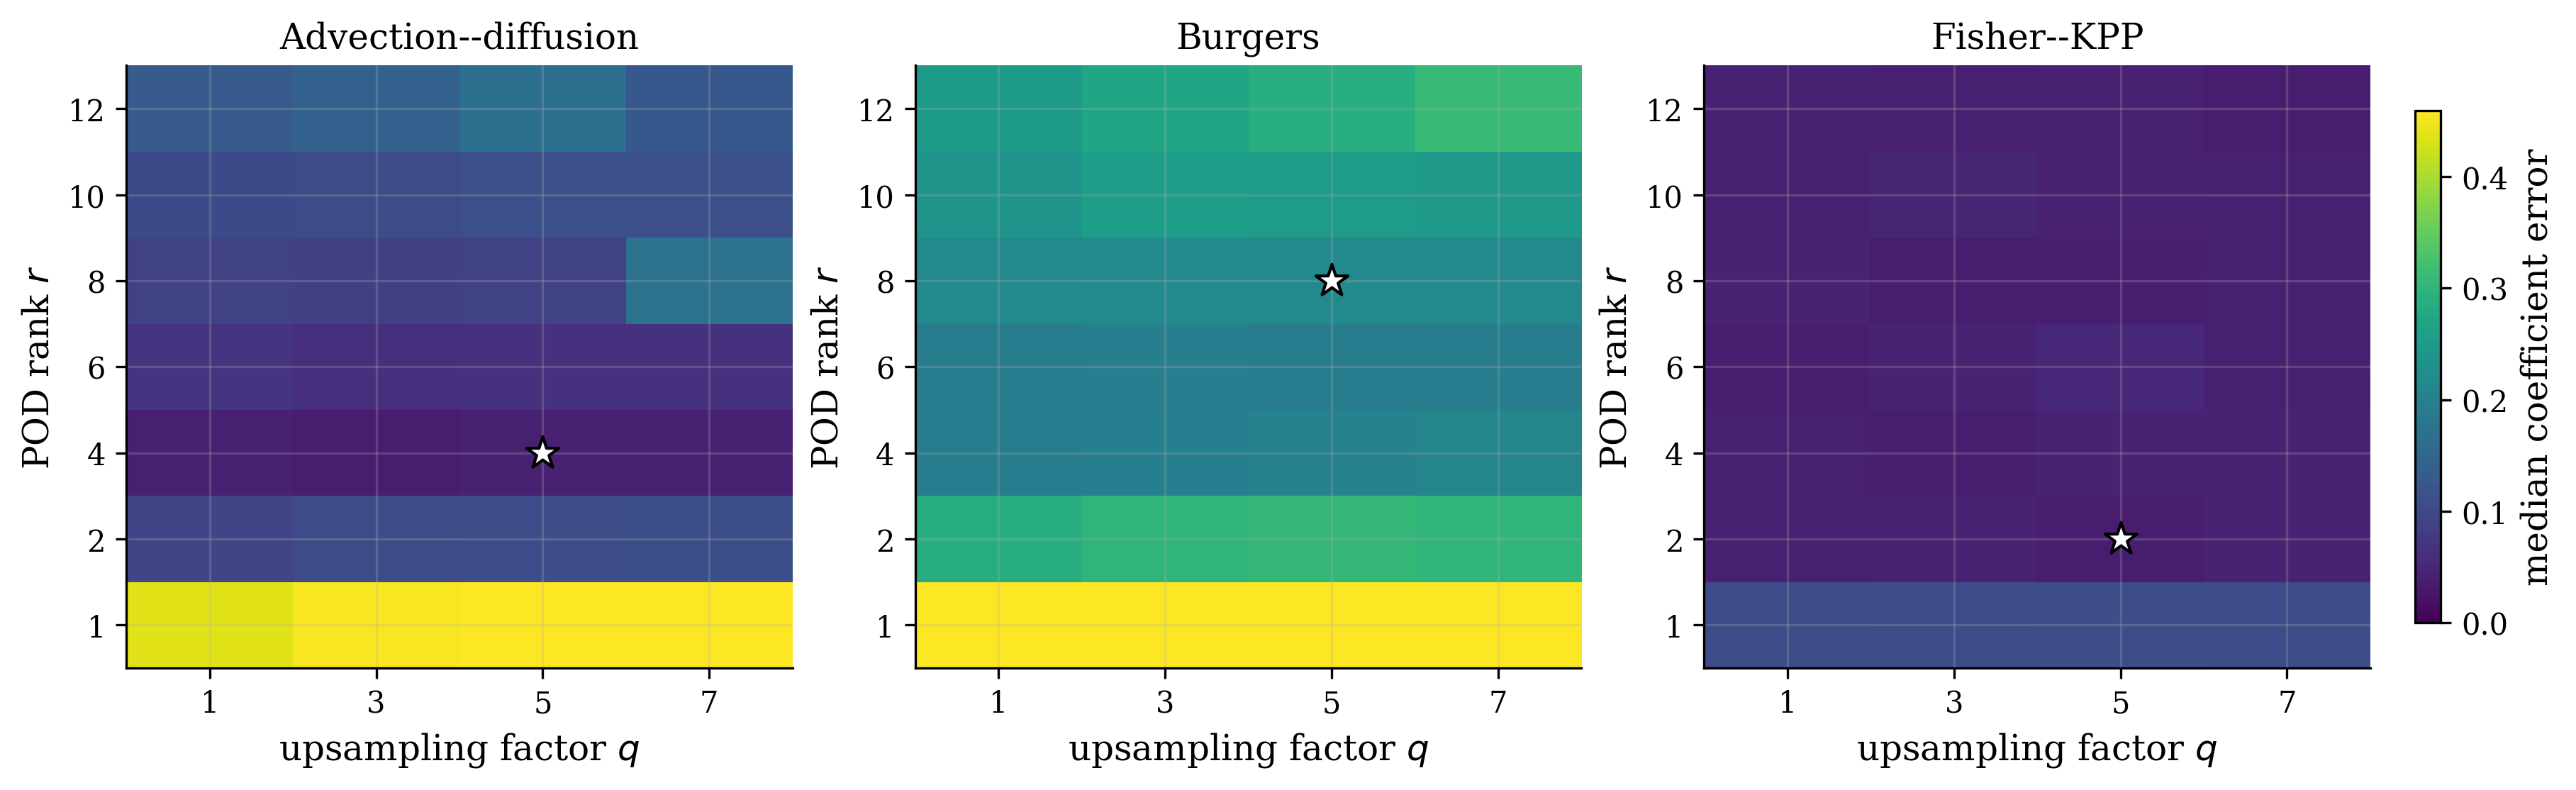
\includegraphics[width=0.95\textwidth]{figures/appendix_qr_sensitivity_pde.png}
\caption{PDE sensitivity of POD-EDMD-RBF preprocessing to the interpolation factor $q$ and POD rank $r$. Each heatmap reports median coefficient error at relative noise 0.03 and PDE sparse factor 8; white stars mark the default values used in the main benchmark. The $q=1$ column corresponds to POD-only denoising without temporal insertion.}
\label{fig:appendix_qr_sensitivity_pde}
\end{figure}

\begin{table}[H]
\centering
\TBL{\caption{Default-versus-best comparison over the PDE $q$--$r$ sensitivity grid for advection--diffusion, Burgers, and Fisher--KPP. The best grid point is selected by mean practical score, with coefficient error used only as a tie-breaker. F1 and practical score are means; coefficient error is the median over five seeds. Boldface marks the better value between the default and best grid point at reported precision.\label{tab:appendix_pde_qr_sensitivity}}}
{\resizebox{\textwidth}{!}{%
\begin{tabular}{@{}lcccccccc@{}}\toprule
\TCH{System} & \multicolumn{4}{c}{\TCH{Default}} & \multicolumn{4}{c}{\TCH{Best}} \\
\cmidrule(lr){2-5}\cmidrule(lr){6-9}
 & \TCH{$(q,r)$} & \TCH{F1} & \TCH{Coeff. err.} & \TCH{Score} & \TCH{$(q,r)$} & \TCH{F1} & \TCH{Coeff. err.} & \TCH{Score} \\ \midrule
Advection--diffusion & (5,4) & \textbf{0.667} & 0.041 & 0.641 & (3,4) & \textbf{0.667} & \textbf{0.035} & \textbf{0.643} \\
Burgers & (5,8) & \textbf{0.667} & 0.220 & 0.545 & (1,6) & \textbf{0.667} & \textbf{0.193} & \textbf{0.559} \\
Fisher--KPP & (5,2) & \textbf{0.800} & \textbf{0.037} & \textbf{0.771} & (7,10) & \textbf{0.800} & 0.041 & \textbf{0.771} \\
\botrule
\end{tabular}%
}}
\end{table}

The PDE grid in Figure~\ref{fig:appendix_qr_sensitivity_pde} and Table~\ref{tab:appendix_pde_qr_sensitivity} supports the use of fixed system-specific ranks in the main study. The $q=1$ column provides the requested POD-only control, while $q>1$ combines the same low-rank spatial projection with temporal upsampling. The default advection--diffusion choice $(q,r)=(5,4)$ is close to the best grid point $(3,4)$; the Burgers default $(5,8)$ is not the lowest-error point in this sensitivity slice but remains in a stable region of the heatmap; and Fisher--KPP has a broad low-error region in which the default rank $r=2$ remains competitive. These results do not imply that $q$ and $r$ are universally optimal. They show that the main conclusions are not based on an isolated unstable choice of interpolation factor or POD rank.
